\section{Hierarchical Methods}

\begin{frame}{Hierarchical Clustering}
	\begin{itemize}
		\item \textbf{Does not require the number of clusters $k$ as an input,
			      \\ but needs a termination condition.}
	\end{itemize}
	\vspace{0.5cm}
	\centering
	\scalebox{0.8}{
		\begin{tikzpicture}[->,>=stealth',auto,node distance=3cm,
				thick,main node/.style={circle,draw}]
			\draw[thick,->] (0,0)--(10,0);
			\draw[thick,->] (10,-4)--(0,-4);
			\draw (1,0)--(1,0.25);
			\node at (1,0.5) {Step 0};
			\draw (3,0)--(3,0.25);
			\node at (3,0.5) {Step 1};
			\draw (5,0)--(5,0.25);
			\node at (5,0.5) {Step 2};
			\draw (7,0)--(7,0.25);
			\node at (7,0.5) {Step 3};
			\draw (9,0)--(9,0.25);
			\node at (9,0.5) {Step 4};
			\draw (1,-4)--(1,-4.25);
			\node at (1,-4.5) {Step 4};
			\draw (3,-4)--(3,-4.25);
			\node at (3,-4.5) {Step 3};
			\draw (5,-4)--(5,-4.25);
			\node at (5,-4.5) {Step 2};
			\draw (7,-4)--(7,-4.25);
			\node at (7,-4.5) {Step 1};
			\draw (9,-4)--(9,-4.25);
			\node at (9,-4.5) {Step 0};
			\node[main node] at (1,-0.5) (a) {a};
			\node[main node] at (1,-1.25) (b) {b};
			\node[main node] at (1,-2) (c) {c};
			\node[main node] at (1,-2.75) (d) {d};
			\node[main node] at (1,-3.5) (e) {e};
			\node[main node] at (3,-0.8) (ab) {a b};
			\node[main node] at (5,-3.2) (de) {d e};
			\node[main node] at (7,-2.5) (cde) {c d e};
			\node[main node] at (9,-1.5) (abcde) {a b c d e};
			\draw (a)--(ab);
			\draw (b)--(ab);
			\draw (ab)--(abcde);
			\draw (c)--(cde);
			\draw (d)--(de);
			\draw (e)--(de);
			\draw (de)--(cde);
			\draw (cde)--(abcde);
			\node at (11.5,-4) {\textbf{divisive (DIANA)}};
			\node at (12,0) {\textbf{agglomerative (AGNES)}};
		\end{tikzpicture}
	}
\end{frame}

\begin{frame}{AGNES (Agglomerative Nesting)}
	\begin{itemize}
		\item \textbf{Introduced in (Kaufmann \& Rousseeuw, 1990)}
		\item \textbf{Use the single-link method.} (see below)
		\item \textbf{Merge nodes that have the least dissimilarity.}
		\item \textbf{Go on in a non-descending fashion.}
		\item \textbf{Eventually all nodes belong to the same cluster.}
	\end{itemize}
	\newcommand*{\xMin}{0}%
	\newcommand*{\xMax}{10}%
	\newcommand*{\yMin}{0}%
	\newcommand*{\yMax}{10}%
	\centering
	\begin{tikzpicture}[scale=0.23]
		\foreach \i in {\xMin,...,\xMax} {
				\draw [very thin,gray] (\i,\yMin) -- (\i,\yMax)  node [below] at
				(\i,\yMin) {\tiny$\i$};
			}
		\foreach \i in {\yMin,...,\yMax} {
				\draw [very thin,gray] (\xMin,\i) -- (\xMax,\i) node [left] at
				(\xMin,\i) {\tiny$\i$};
			}
		\node[color=orange] at (2,6) {\Huge\textbullet};
		\node[color=orange] at (3,4) {\Huge\textbullet};
		\node[color=orange] at (3,8) {\Huge\textbullet};
		\node[color=orange] at (4,5) {\Huge\textbullet};
		\node[color=orange] at (4,7) {\Huge\textbullet};
		\node[color=orange] at (6,2) {\Huge\textbullet};
		\node[color=orange] at (7,2) {\Huge\textbullet};
		\node[color=orange] at (7,4) {\Huge\textbullet};
		\node[color=orange] at (8,4) {\Huge\textbullet};
		\node[color=orange] at (8,5) {\Huge\textbullet};
		\draw[->] (12,5)--(17,5);
		\draw[dashed] (3.4,7.5) ellipse (1.5cm and 1.2cm);
		\draw[dashed] (3.5,4.8) ellipse (1.5cm and 1cm);
		\draw[dashed] (8,5) ellipse (1cm and 1.5cm);
	\end{tikzpicture}
	\begin{tikzpicture}[scale=0.23]
		\foreach \i in {\xMin,...,\xMax} {
				\draw [very thin,gray] (\i,\yMin) -- (\i,\yMax)  node [below] at
				(\i,\yMin) {\tiny$\i$};
			}
		\foreach \i in {\yMin,...,\yMax} {
				\draw [very thin,gray] (\xMin,\i) -- (\xMax,\i) node [left] at
				(\xMin,\i) {\tiny$\i$};
			}
		\node[color=orange] at (2,6) {\Huge\textbullet};
		\node[color=orange] at (3,4) {\Huge\textbullet};
		\node[color=orange] at (3,8) {\Huge\textbullet};
		\node[color=orange] at (4,5) {\Huge\textbullet};
		\node[color=orange] at (4,7) {\Huge\textbullet};
		\node[color=orange] at (6,2) {\Huge\textbullet};
		\node[color=orange] at (7,2) {\Huge\textbullet};
		\node[color=orange] at (7,4) {\Huge\textbullet};
		\node[color=orange] at (8,4) {\Huge\textbullet};
		\node[color=orange] at (8,5) {\Huge\textbullet};
		\draw[->] (12,5)--(17,5);
		\draw[dashed] (3,7) ellipse (2cm and 1.5cm);
		\draw[dashed] (3.5,4.8) ellipse (1.5cm and 1cm);
		\draw[dashed] (7.5,5) ellipse (1.5cm and 1.5cm);
		\draw[dashed] (6.25,2.5) ellipse (1.5cm and 1cm);
	\end{tikzpicture}
	\begin{tikzpicture}[scale=0.23]
		\foreach \i in {\xMin,...,\xMax} {
				\draw [very thin,gray] (\i,\yMin) -- (\i,\yMax)  node [below] at
				(\i,\yMin) {\tiny$\i$};
			}
		\foreach \i in {\yMin,...,\yMax} {
				\draw [very thin,gray] (\xMin,\i) -- (\xMax,\i) node [left] at
				(\xMin,\i) {\tiny$\i$};
			}
		\node[color=orange] at (2,6) {\Huge\textbullet};
		\node[color=orange] at (3,4) {\Huge\textbullet};
		\node[color=orange] at (3,8) {\Huge\textbullet};
		\node[color=orange] at (4,5) {\Huge\textbullet};
		\node[color=orange] at (4,7) {\Huge\textbullet};
		\node[color=orange] at (6,2) {\Huge\textbullet};
		\node[color=orange] at (7,2) {\Huge\textbullet};
		\node[color=orange] at (7,4) {\Huge\textbullet};
		\node[color=orange] at (8,4) {\Huge\textbullet};
		\node[color=orange] at (8,5) {\Huge\textbullet};
		\draw[dashed] (3,6) ellipse (2cm and 3cm);
		\draw[dashed] (7,4) ellipse (2cm and 3cm);
	\end{tikzpicture}
\end{frame}

\begin{frame}{Dendrogram: Shows how Clusters are Merged}
	\begin{itemize}
		\item Decompose data objects into a several levels of nested
		      partitioning (tree of clusters),\\ called a
		      \textbf{\color{airforceblue}dendrogram}.
		\item A clustering of the data objects is obtained by
		      \textbf{\color{airforceblue}cutting} the dendrogram at the desired
		      level,\\ then each connected component forms a cluster.
	\end{itemize}
	\centering
	\resizebox{6.7cm}{!}{%
		\begin{tikzpicture}[sloped]
			\node (a) at (-6,0) {a};
			\node (b) at (-3,0) {b};
			\node (c) at (-0.5,0) {c};
			\node (d) at (0.5,0) {d};
			\node (e) at (2,0) {e};
			\node (ab) at (-4.5,3) {};
			\node (cd) at (0,1) {};
			\node (cde) at (1,2) {};
			\node (all) at (-1.5,5) {};

			\draw  (a) |- (ab.center);
			\draw  (b) |- (ab.center);
			\draw  (c) |- (cd.center);
			\draw  (d) |- (cd.center);
			\draw  (e) |- (cde.center);
			\draw  (cd.center) |- (cde.center);
			\draw  (ab.center) |- (all.center);
			\draw  (cde.center) |- (all.center);

			\draw[->,-triangle 60] (-7,0) -- node[above]{distance} (-7,6);
		\end{tikzpicture}}
\end{frame}

\begin{frame}{DIANA (Divisive Analysis)}
	\begin{itemize}
		\item \textbf{Introduced in (Kaufmann \& Rousseeuw, 1990)}
		\item \textbf{Inverse order of AGNES.}
		\item \textbf{Eventually each node forms a cluster of its own.}
	\end{itemize}
	\newcommand*{\xMin}{0}%
	\newcommand*{\xMax}{10}%
	\newcommand*{\yMin}{0}%
	\newcommand*{\yMax}{10}%
	\vspace{0.5cm}
	\centering
	\begin{tikzpicture}[scale=0.23]
		\foreach \i in {\xMin,...,\xMax} {
				\draw [very thin,gray] (\i,\yMin) -- (\i,\yMax)  node [below] at
				(\i,\yMin) {\tiny$\i$};
			}
		\foreach \i in {\yMin,...,\yMax} {
				\draw [very thin,gray] (\xMin,\i) -- (\xMax,\i) node [left] at
				(\xMin,\i) {\tiny$\i$};
			}
		\node[color=orange] at (2,6) {\Huge\textbullet};
		\node[color=orange] at (3,4) {\Huge\textbullet};
		\node[color=orange] at (3,8) {\Huge\textbullet};
		\node[color=orange] at (4,5) {\Huge\textbullet};
		\node[color=orange] at (4,7) {\Huge\textbullet};
		\node[color=orange] at (6,2) {\Huge\textbullet};
		\node[color=orange] at (7,2) {\Huge\textbullet};
		\node[color=orange] at (7,4) {\Huge\textbullet};
		\node[color=orange] at (8,4) {\Huge\textbullet};
		\node[color=orange] at (8,5) {\Huge\textbullet};
		\draw[->] (12,5)--(17,5);
		\draw[dashed] (3,6) ellipse (2cm and 3cm);
		\draw[dashed] (7,4) ellipse (2cm and 3cm);
	\end{tikzpicture}
	\begin{tikzpicture}[scale=0.23]
		\foreach \i in {\xMin,...,\xMax} {
				\draw [very thin,gray] (\i,\yMin) -- (\i,\yMax)  node [below] at
				(\i,\yMin) {\tiny$\i$};
			}
		\foreach \i in {\yMin,...,\yMax} {
				\draw [very thin,gray] (\xMin,\i) -- (\xMax,\i) node [left] at
				(\xMin,\i) {\tiny$\i$};
			}
		\node[color=orange] at (2,6) {\Huge\textbullet};
		\node[color=orange] at (3,4) {\Huge\textbullet};
		\node[color=orange] at (3,8) {\Huge\textbullet};
		\node[color=orange] at (4,5) {\Huge\textbullet};
		\node[color=orange] at (4,7) {\Huge\textbullet};
		\node[color=orange] at (6,2) {\Huge\textbullet};
		\node[color=orange] at (7,2) {\Huge\textbullet};
		\node[color=orange] at (7,4) {\Huge\textbullet};
		\node[color=orange] at (8,4) {\Huge\textbullet};
		\node[color=orange] at (8,5) {\Huge\textbullet};
		\draw[->] (12,5)--(17,5);
		\draw[dashed] (3,7) ellipse (2cm and 1.5cm);
		\draw[dashed] (3.5,4.8) ellipse (1.5cm and 1cm);
		\draw[dashed] (7.5,5) ellipse (1.5cm and 1.5cm);
		\draw[dashed] (6.25,2.5) ellipse (1.5cm and 1cm);
	\end{tikzpicture}
	\begin{tikzpicture}[scale=0.23]
		\foreach \i in {\xMin,...,\xMax} {
				\draw [very thin,gray] (\i,\yMin) -- (\i,\yMax)  node [below] at
				(\i,\yMin) {\tiny$\i$};
			}
		\foreach \i in {\yMin,...,\yMax} {
				\draw [very thin,gray] (\xMin,\i) -- (\xMax,\i) node [left] at
				(\xMin,\i) {\tiny$\i$};
			}
		\node[color=orange] at (2,6) {\Huge\textbullet};
		\node[color=orange] at (3,4) {\Huge\textbullet};
		\node[color=orange] at (3,8) {\Huge\textbullet};
		\node[color=orange] at (4,5) {\Huge\textbullet};
		\node[color=orange] at (4,7) {\Huge\textbullet};
		\node[color=orange] at (6,2) {\Huge\textbullet};
		\node[color=orange] at (7,2) {\Huge\textbullet};
		\node[color=orange] at (7,4) {\Huge\textbullet};
		\node[color=orange] at (8,4) {\Huge\textbullet};
		\node[color=orange] at (8,5) {\Huge\textbullet};
		\draw[dashed] (3.4,7.5) ellipse (1.5cm and 1.2cm);
		\draw[dashed] (3.5,4.8) ellipse (1.5cm and 1cm);
		\draw[dashed] (8,5) ellipse (1cm and 1.5cm);
		\draw[dashed] (7,4.3) ellipse (0.8cm and 0.8cm);
		\draw[dashed] (6.25,2.5) ellipse (1.5cm and 1cm);
		\draw[dashed] (2,6) ellipse (0.8cm and 0.8cm);
	\end{tikzpicture}
\end{frame}

\begin{frame}{Distance Between Clusters (I)}
	\begin{itemize}
		\item \textbf{Minimum distance:}
		      \begin{itemize}
			      \item Smallest distance between an object in one cluster and an
			            object in the other, i.e., $\text{dist}_{\text{min}} (C_i, C_j) =
				            \text{min}_{o_{ip} \in C_i, o_{jq} \in C_j} d(o_{ip}, o_{jq})$.
		      \end{itemize}
		\item \textbf{Maximum distance:}
		      \begin{itemize}
			      \item Largest distance between an object in one cluster and an
			            object in the other, i.e., $\text{dist}_\text{max}(C_i, C_j) =
				            \text{max}_{o_{ip} \in C_i, o_{jq} \in C_j} d(o_{ip}, o_{jq}).$
		      \end{itemize}
		\item \textbf{Average distance:}
		      \begin{itemize}
			      \item Average distance between an object in one cluster and an
			            object in the other, i.e., $\text{dist}_{\text{avg}} (C_i, C_j) =
				            \frac{1}{n_i \cdot n_j} \sum_{o_{ip} \in C_i, o_{jq} \in C_j}
				            d(o_{ip}, o_{jq}).$
		      \end{itemize}
		\item \textbf{Mean distance:}
		      \begin{itemize}
			      \item Distance between the centroids of two clusters, i.e.,
			            $\text{dist}_{\text{mean}} (C_i, C_j) = d(c_i, c_j).$
		      \end{itemize}
	\end{itemize}
\end{frame}

\begin{frame}{Distance between Clusters (II)}
	\begin{itemize}
		\item \textbf{Nearest-neighbor clustering algorithm:}
		      \begin{itemize}
			      \item Uses \textbf{\color{airforceblue}minimum distance} to measure
			            distance between clusters.
		      \end{itemize}
		\item \textbf{Single-linkage algorithm:}
		      \begin{itemize}
			      \item Terminates if distance between nearest clusters exceeds
			            user-defined threshold.
		      \end{itemize}
		\item \textbf{Minimal spanning-tree algorithm:}
		      \begin{itemize}
			      \item View objects (data points) as nodes of a graph.
			      \item Edges form a path between nodes in a cluster.
			      \item Merging of two clusters corresponds to adding an edge between
			            the nearest pair of nodes.
			      \item Because edges linking clusters always go between distinct
			            clusters,\\
			            resulting graph will be a tree.
			      \item Thus, agglomerative hierarchical clustering that uses minimum
			            distance produces minimal spanning tree.
		      \end{itemize}
	\end{itemize}
\end{frame}

\begin{frame}{Distance between Clusters (III)}
	\begin{itemize}
		\item \textbf{Farthest-neighbor clustering algorithm:}
		      \begin{itemize}
			      \item Uses \textbf{\color{airforceblue}maximum distance} to measure
			            distance between clusters.
		      \end{itemize}
		\item \textbf{Complete-linkage algorithm:}
		      \begin{itemize}
			      \item Terminates if maximum distance between nearest clusters
			            exceeds user-defined threshold.
			      \item Good if true clusters are rather compact and approx. equal in
			            size.
		      \end{itemize}
	\end{itemize}
\end{frame}

\begin{frame}{Extensions to Hierarchical Clustering}
	\begin{itemize}
		\item \textbf{Major weakness of agglomerative clustering methods:}
		      \begin{itemize}
			      \item Can never undo what was done previously.
			      \item Do not scale well: Time complexity of at least
			            $\mathcal{O}(n^2)$, where $n$ is the number of objects.
		      \end{itemize}
		\item \textbf{Integration of hierarchical and distance-based
			      clustering:}
		      \begin{itemize}
			      \item BIRCH (1996): Uses CF-tree and incrementally adjusts the
			            quality of sub-clusters.
			      \item CHAMELEON (1999): Hierarchical clustering using dynamic
			            modeling.
		      \end{itemize}
	\end{itemize}
\end{frame}

\begin{frame}{BIRCH (Balanced Iterative Reducing and Clustering Using
		Hierarchies)}
	(Zhang, Ramakrishnan \& Livny, SIGMOD'96)

	\textbf{Incrementally construct a CF (Clustering Feature) tree:}
	\begin{itemize}
		\item A hierarchical data structure for multiphase clustering.
		\item Phase 1: Scan DB to build an initial in-memory CF-tree.
		      \begin{itemize}
			      \item A multi-level compression of the data that tries to
			            preserve the inherent clustering structure of the data.
		      \end{itemize}
		\item Phase 2: Use an arbitrary clustering algorithm to cluster the
		      leaf nodes of the CF-tree.
	\end{itemize}
	\textbf{Scales linearly:}
	\begin{itemize}
		\item Finds a good clustering with a single scan and improves the
		      quality with a few additional scans.
	\end{itemize}
	\textbf{Weakness:}
	\begin{itemize}
		\item Handles only numerical data, and sensitive to the order of
		      the data records.
	\end{itemize}
\end{frame}

\begin{frame}{Clustering Feature in BIRCH}
	\textbf{Clustering Feature CF = (n, LS, SS)}:
	\begin{itemize}
		\item $3$D vector summarizing statistics about clusters:
		      \begin{itemize}
			      \item $n$: number of data points.
			      \item LS: linear sum of $N$ points $\sum_{i=1}^{n} x_i$.
			      \item SS: square sum of $N$ points $\sum_{i=1}^{n} x_i^2$.
		      \end{itemize}
	\end{itemize}
	\newcommand*{\xMin}{0}%
	\newcommand*{\xMax}{10}%
	\newcommand*{\yMin}{0}%
	\newcommand*{\yMax}{10}%
	\centering
	\scalebox{0.9}{
		\begin{tikzpicture}[scale=0.3]
			\foreach \i in {\xMin,...,\xMax} {
					\draw [very thin,gray] (\i,\yMin) -- (\i,\yMax)  node [below]
					at
					(\i,\yMin) {\tiny$\i$};
				}
			\foreach \i in {\yMin,...,\yMax} {
					\draw [very thin,gray] (\xMin,\i) -- (\xMax,\i) node [left] at
					(\xMin,\i) {\tiny$\i$};
				}
			\node[color=orange] at (2,6) {\Huge\textbullet};
			\node[color=orange] at (3,4) {\Huge\textbullet};
			\node[color=orange] at (3,8) {\Huge\textbullet};
			\node[color=orange] at (4,5) {\Huge\textbullet};
			\node[color=orange] at (4,7) {\Huge\textbullet};
			\node[color=orange] at (6,2) {\Huge\textbullet};
			\node[color=orange] at (7,2) {\Huge\textbullet};
			\node[color=orange] at (7,4) {\Huge\textbullet};
			\node[color=orange] at (8,4) {\Huge\textbullet};
			\node[color=orange] at (8,5) {\Huge\textbullet};
			\draw[dashed] (3,6) ellipse (2cm and 3cm);
			\draw[dashed] (7,4) ellipse (2cm and 3cm);
			\node[draw] at (18,9) {CF = $(5,(16,30),(54,190))$};
			\node at (18,7) {\small as the data points contained are:};
			\node at (18,5.7) {(3,4),(2,6),(4,5),(4,7),(3,8)};
			\draw[->] (16,10) to [out=30,in=30] (3.3,9.5);
		\end{tikzpicture}
	}
\end{frame}

\begin{frame}{Clustering Feature in BIRCH (II)}
	\begin{itemize}
		\item \textbf{Allows to derive many useful statistics of a cluster. E.g.:}
		      \begin{itemize}
			      \item centroid: $c = \frac{\sum_{i=1}^{n}o_i}{n} = \frac{LS}{n}$,
			      \item radius: $R = \sqrt{\frac{\sum_{i=1}^{n}(x_i-c)^2}{n}} = \sqrt{\frac{nSS-2LS^2+nLS}{n^2}}$,
			      \item diameter: $D = \sqrt{\frac{\sum_{i=1}^{n}\sum_{j=1}^{n}(x_i-x_j)^2}{n(n-1)}} = \sqrt{\frac{2nSS-2LS^2}{n(n-1)}}$
		      \end{itemize}
		\item \textbf{Additive:}
		      \begin{itemize}
			      \item For two disjoint clusters $C_1$ and $C_2$ with clustering
			            features $CF_1 = (n_1, LS_1, SS_1)$ and $CF_2 = (n_2, LS_2, SS_2)$,
			            the clustering feature of the cluster that is formed by merging
			            $C_1$ and $C_2$ is simply: $CF_1 + CF_2 = (n_1 + n_2, LS_1 + LS_2, SS_1 + SS_2)$.
		      \end{itemize}
	\end{itemize}
\end{frame}

\begin{frame}{CF-Tree in BIRCH}
	\begin{itemize}
		\item \textbf{Height-balanced tree.}
		\item \textbf{Stores the clustering features for a hierarchical
			      clustering.}
		      \begin{itemize}
			      \item Non-leaf nodes store sums of the CFs of their children.
		      \end{itemize}
		\item \textbf{Two parameters:}
		      \begin{itemize}
			      \item \textbf{\color{airforceblue}Branching factor $B$}: max \# of
			            children.
			      \item \textbf{\color{airforceblue}Threshold $T$}: maximum diameter
			            of sub-clusters stored at leaf nodes.

			            \begin{itemize}

				            \item Diameter $D$: average pairwise distance within a cluster, \\
				                  reflects the tightness of the cluster around the centroid:
				                  \begin{align*}
					                  D = \sqrt{\frac{\sum_{i=1}^{n} \sum_{j=1}^{n}
							                  (o_i-o_j)^2}{n(n-1)}} = \sqrt{\frac{2nSS - 2LS^2}{n(n-1)}}.
				                  \end{align*}

			            \end{itemize}

		      \end{itemize}
	\end{itemize}
\end{frame}

\begin{frame}{CF-Tree structure}
	\centering
	\begin{tikzpicture}
		\node at (0,0.75) {Root:};
		\node at (0,0) {
			\begin{tabular}{|c|c|c|c|c|}
				\hline
				$CF_1$           & $CF_2$           & $CF_3$           &
				$\hdots$         & $CF_6$                                \\ \hline
				$\text{child}_1$ & $\text{child}_2$ & $\text{child}_3$ &
				$\hdots$         & $\text{child}_6$                      \\\hline
			\end{tabular}
		};
		\node at (-2,-1.2) {Non-leaf node:};
		\node at (-2,-2) {
			\begin{tabular}{|c|c|c|c|c|}
				\hline
				$CF_{11}$           & $CF_{12}$           & $CF_{13}$
				                    & $\hdots$            & $CF_{15}$           \\ \hline
				$\text{child}_{11}$ & $\text{child}_{12}$ & $\text{child}_{13}$
				                    & $\hdots$            & $\text{child}_{15}$ \\\hline
			\end{tabular}
		};
		\node at (3,-2) {$\hdots$};
		\node at (5,-2) {$\hdots$};
		\node at (-3,-3.5) {Leaf node:};
		\node at (-3,-4) {
			\begin{tabular}{|c|c|c|c|c|c|}
				\hline
				prev & $CF_{111}$ & $CF_{112}$ & $\hdots$ & $CF_{116}$ & next
				\\ \hline
			\end{tabular}
		};
		\node at (4,-3.5) {Leaf node:};
		\node at (4,-4) {
			\begin{tabular}{|c|c|c|c|c|c|}
				\hline
				prev & $CF_{121}$ & $CF_{122}$ & $\hdots$ & $CF_{124}$ & next
				\\ \hline
			\end{tabular}
		};
		\draw[thick,->] (-2.2,-0.45)--(-4.3,-1.5);
		\draw[thick,->] (-1.2,-0.45)--(2.3,-1.5);
		\draw[thick,->] (0.2,-0.45)--(4.3,-1.5);
		\draw[thick,->] (-3,-2.45)--(2.3,-3.7);
		\draw[thick,->] (-4.3,-2.45)--(-5.2,-3.7);
		\draw[thick,->] (0.1,-3.6)--(0.9,-3.6);
		\draw[thick,->] (0.9,-4.4)--(0.1,-4.4);
		\draw[thick,->] (7.1,-3.6)--(7.9,-3.6);
		\draw[thick,->] (7.9,-4.4)--(7.1,-4.4);
		\node at (-5,0) {B=7};
		\node at (-5,-0.5) {T=6};
	\end{tikzpicture}
\end{frame}

\begin{frame}{The BIRCH algorithm}
	\textbf{Phase 1:}
	\begin{itemize}
		\item \textbf{For each point in the input:}
		      \begin{itemize}
			      \item Find closest leaf-node entry.
			      \item Add point to leaf-node entry and update CF.
			      \item If $entry\_diameter > max\_diameter$, then split leaf
			            node, and possibly parents.
			      \item Information about new point is passed toward the root of
			            the tree.
		      \end{itemize}
		\item \textbf{Algorithm is $\mathcal{O}(n)$ and incremental.}
		\item \textbf{Concerns:}
		      \begin{itemize}
			      \item Sensitive to insertion order of data points.
			      \item Since we fix the size of leaf nodes, clusters may not be
			            so natural.
			      \item Clusters tend to be spherical given the radius and
			            diameter measures.
		      \end{itemize}
	\end{itemize}
\end{frame}

\begin{frame}{CHAMELEON: Hierarchical Clustering using Dynamic Modeling}

	(Karypis, Han \& Kumar, 1999)
	\begin{itemize}
		\item \textbf{Measures the similarity based on a dynamic model:}
		      \begin{itemize}
			      \item Two clusters are merged only if the
			            \textbf{interconnectivity} and \textbf{closeness (proximity)}
			            between two clusters are high relative to the intraconnectivity
			            of the clusters and the closeness of items within the clusters.
		      \end{itemize}
		\item \textbf{Graph-based, and a two-phase algorithm.}
		      \begin{itemize}
			      \item Use a graph-partitioning algorithm:
			            \begin{itemize}
				            \item Cluster objects into a large number of relatively
				                  small sub-clusters.
			            \end{itemize}
			      \item Use an agglomerative hierarchical clustering algorithm:
			            \begin{itemize}
				            \item Find the genuine clusters by repeatedly combining
				                  these sub-clusters.
			            \end{itemize}
		      \end{itemize}
	\end{itemize}

\end{frame}

\begin{frame}{Overall Framework of CHAMELEON}
	\centering
	\scalebox{0.85}{
		\begin{tikzpicture}[scale=0.9, node distance = 1cm,
				auto,font=\footnotesize,
				force/.style={rectangle, draw, fill=black!10, inner sep=5pt, text
						width=1.8cm, text badly centered, minimum height=1cm,
						font=\bfseries\footnotesize\sffamily},
				info/.style={rectangle, draw, inner sep=5pt, text width=4cm,
						minimum
						height=1cm, font=\footnotesize\sffamily}]
			\node [force, dashed] (a) {\parbox{\linewidth}{\centering Data \\
					input.}};

			\node[draw, circle, fill=black, scale=0.4] at (4,0) (g1) {};
			\node[draw, circle, fill=black, scale=0.4] at (4.3,0.3) (g2) {};
			\node[draw, circle, fill=black, scale=0.4] at (4.4,-0.2) (g3) {};
			\node[draw, circle, fill=black, scale=0.4] at (4,-0.4) (g4) {};
			\draw[color=black] (g1)--(g2)--(g3)--(g4)--(g1);
			\draw[color=black] (g1)--(g3);
			\draw[color=black] (g2)--(g4);

			\node[draw, circle, fill=black, scale=0.4] at (5.5,0.5) (y1) {};
			\node[draw, circle, fill=black, scale=0.4] at (6,0.8) (y2) {};
			\node[draw, circle, fill=black, scale=0.4] at (6,0.3) (y3) {};
			\node[draw, circle, fill=black, scale=0.4] at (5.7,0.1) (y4) {};
			\draw[color=black] (y1)--(y2)--(y3)--(y4)--(y1);
			\draw[color=black] (y1)--(y3);
			\draw[color=black] (y2)--(y4);

			\node[draw, circle, fill=black, scale=0.4] at (6.7,-0.7) (sch1) {};
			\node[draw, circle, fill=black, scale=0.4] at (6.4,-1) (sch2) {};
			\node[draw, circle, fill=black, scale=0.4] at (6.8,-1.2) (sch3) {};
			\draw[color=black] (sch1)--(sch2)--(sch3)--(sch1);

			\node[draw, circle, fill=black, scale=0.4] at (3.7,-1) (b1) {};
			\node[draw, circle, fill=black, scale=0.4] at (3.4,-1.1) (b2) {};
			\node[draw, circle, fill=black, scale=0.4] at (3.8,-1.3) (b3) {};
			\draw[color=black] (b1)--(b2)--(b3)--(b1);
			\draw (g1)--(b2);
			\draw (g4)--(b3);

			\node[draw, circle, fill=black, scale=0.4] at (5,-0.6) (r1) {};
			\node[draw, circle, fill=black, scale=0.4] at (5.2,-0.5) (r2) {};
			\node[draw, circle, fill=black, scale=0.4] at (5.5,-1) (r3) {};
			\node[draw, circle, fill=black, scale=0.4] at (5.2,-0.9) (r4) {};
			\node[draw, circle, fill=black, scale=0.4] at (5.3,-1.2) (r5) {};
			\draw[color=black] (r1)--(r2)--(r3)--(r4)--(r5);
			\draw[color=black] (r1)--(r3);
			\draw[color=black] (r1)--(r4);
			\draw[color=black] (r2)--(r4);
			\draw[color=black] (r3)--(r5);

			\node[draw, circle, fill=black, scale=0.4] at (4.5,-1.5) (p1) {};
			\node[draw, circle, fill=black, scale=0.4] at (5,-1.9) (p2) {};
			\node[draw, circle, fill=black, scale=0.4] at (4.1,-1.9) (p3) {};
			\node[draw, circle, fill=black, scale=0.4] at (4.9,-2.4) (p4) {};
			\node[draw, circle, fill=black, scale=0.4] at (4,-2.4) (p5) {};
			\node[draw, circle, fill=black, scale=0.4] at (4.5,-2.1) (p6) {};
			\draw[color=black] (p1)--(p2);
			\draw[color=black] (p1)--(p3);
			\draw[color=black] (p4)--(p6);
			\draw[color=black] (p4)--(p5);
			\draw[color=black] (p5)--(p6);
			\draw[color=black] (p6)--(p1);
			\draw[color=black] (p2)--(p3);
			\draw[color=black] (p2)--(p4);
			\draw[color=black] (p2)--(p6);
			\draw[color=black] (p5)--(p3);
			\draw[color=black] (p3)--(p6);
			\draw (b3)--(p3);
			\draw (g4)--(p1);
			\draw (g2)--(p2);
			\draw (g2)--(p1);
			\draw (r1)--(p2);
			\draw (r5)--(p2);
			\draw (y1)--(r1);
			\draw (y4)--(r2);

			\node[draw, circle, fill=black, scale=0.4] at (6,-2.5) (o1) {};
			\node[draw, circle, fill=black, scale=0.4] at (6.3,-2.8) (o2) {};
			\node[draw, circle, fill=black, scale=0.4] at (6.3,-2.5) (o3) {};
			\node[draw, circle, fill=black, scale=0.4] at (5.9,-2.8) (o4) {};
			\draw[color=black] (o1)--(o2)--(o3)--(o4)--(o1);
			\draw[color=black] (o2)--(o4);
			\draw[color=black] (o3)--(o1);

			\node[draw, circle, fill=black, scale=0.4] at (6,-1.6) (b1) {};
			\node[draw, circle, fill=black, scale=0.4] at (6.3,-1.9) (b2) {};
			\node[draw, circle, fill=black, scale=0.4] at (6.3,-1.6) (b3) {};
			\draw[color=black] (b1)--(b2)--(b3)--(b1);

			\node[draw, circle, fill=green, scale=0.4] at (10,0) (cg1) {};
			\node[draw, circle, fill=green, scale=0.4] at (10.3,0.3) (cg2) {};
			\node[draw, circle, fill=green, scale=0.4] at (10.4,-0.2) (cg3) {};
			\node[draw, circle, fill=green, scale=0.4] at (10,-0.4) (cg4) {};
			\draw[color=green] (cg1)--(cg2)--(cg3)--(cg4)--(cg1);
			\draw[color=green] (cg1)--(cg3);
			\draw[color=green] (cg2)--(cg4);

			\node[draw, circle, fill=yellow, scale=0.4] at (11.5,0.5) (cy1) {};
			\node[draw, circle, fill=yellow, scale=0.4] at (12,0.8) (cy2) {};
			\node[draw, circle, fill=yellow, scale=0.4] at (12,0.3) (cy3) {};
			\node[draw, circle, fill=yellow, scale=0.4] at (11.7,0.1) (cy4) {};
			\draw[color=yellow] (cy1)--(cy2)--(cy3)--(cy4)--(cy1);
			\draw[color=yellow] (cy1)--(cy3);
			\draw[color=yellow] (cy2)--(cy4);

			\node[draw, circle, fill=black, scale=0.4] at (12.7,-0.7) (csch1)
			{};
			\node[draw, circle, fill=black, scale=0.4] at (12.4,-1) (csch2) {};
			\node[draw, circle, fill=black, scale=0.4] at (12.8,-1.2) (csch3)
			{};
			\draw[color=black] (csch1)--(csch2)--(csch3)--(csch1);

			\node[draw, circle, fill=blue, scale=0.4] at (9.7,-1) (cb1) {};
			\node[draw, circle, fill=blue, scale=0.4] at (9.4,-1.1) (cb2) {};
			\node[draw, circle, fill=blue, scale=0.4] at (9.8,-1.3) (cb3) {};
			\draw[color=blue] (cb1)--(cb2)--(cb3)--(cb1);

			\node[draw, circle, fill=red, scale=0.4] at (11,-0.6) (cr1) {};
			\node[draw, circle, fill=red, scale=0.4] at (11.2,-0.5) (cr2) {};
			\node[draw, circle, fill=red, scale=0.4] at (11.5,-1) (cr3) {};
			\node[draw, circle, fill=red, scale=0.4] at (11.2,-0.9) (cr4) {};
			\node[draw, circle, fill=red, scale=0.4] at (11.3,-1.2) (cr5) {};
			\draw[color=red] (cr1)--(cr2)--(cr3)--(cr4)--(cr5);
			\draw[color=red] (cr1)--(cr3);
			\draw[color=red] (cr1)--(cr4);
			\draw[color=red] (cr2)--(cr4);
			\draw[color=red] (cr3)--(cr5);

			\node[draw, circle, fill=purple, scale=0.4] at (10.5,-1.5) (cp1) {};
			\node[draw, circle, fill=purple, scale=0.4] at (11,-1.9) (cp2) {};
			\node[draw, circle, fill=purple, scale=0.4] at (10.1,-1.9) (cp3) {};
			\node[draw, circle, fill=purple, scale=0.4] at (10.9,-2.4) (cp4) {};
			\node[draw, circle, fill=purple, scale=0.4] at (10,-2.4) (cp5) {};
			\node[draw, circle, fill=purple, scale=0.4] at (10.5,-2.1) (cp6) {};
			\draw[color=purple] (cp1)--(cp2);
			\draw[color=purple] (cp1)--(cp3);
			\draw[color=purple] (cp4)--(cp6);
			\draw[color=purple] (cp4)--(cp5);
			\draw[color=purple] (cp5)--(cp6);
			\draw[color=purple] (cp6)--(cp1);
			\draw[color=purple] (cp2)--(cp3);
			\draw[color=purple] (cp2)--(cp4);
			\draw[color=purple] (cp2)--(cp6);
			\draw[color=purple] (cp5)--(cp3);
			\draw[color=purple] (cp3)--(cp6);

			\node[draw, circle, fill=orange, scale=0.4] at (12,-2.5) (co1) {};
			\node[draw, circle, fill=orange, scale=0.4] at (12.3,-2.8) (co2) {};
			\node[draw, circle, fill=orange, scale=0.4] at (12.3,-2.5) (co3) {};
			\node[draw, circle, fill=orange, scale=0.4] at (11.9,-2.8) (co4) {};
			\draw[color=orange] (co1)--(co2)--(co3)--(co4)--(co1);
			\draw[color=orange] (co2)--(co4);
			\draw[color=orange] (co3)--(co1);

			\node[draw, circle, fill=brown, scale=0.4] at (12,-1.6) (cb1) {};
			\node[draw, circle, fill=brown, scale=0.4] at (12.3,-1.9) (cb2) {};
			\node[draw, circle, fill=brown, scale=0.4] at (12.3,-1.6) (cb3) {};
			\draw[color=brown] (cb1)--(cb2)--(cb3)--(cb1);

			\node[draw, info] at (0,-5) {\parbox{\linewidth}{\centering
					\textbf{$k$-NN graph:} \\ $p$ and $q$ are connected if $q$ \\ is
					among
					the top $k$ closest \\ neighbors of $p$.}};
			\node[draw, info] at (11.5,-5) {\parbox{\linewidth}{\centering
					\textbf{Relative interconnectivity:} \\ connectivity of $C_1$ and
					$C_2$
					\\ over internal connectivity. \\[0.2cm] \textbf{Relative
						closeness:}
					\\ closeness of $C_1$ and $C_2$ over \\ internal closeness.}};
			\draw[thick,->] (1.5,0)--(3.5,0);
			\node at (2.5,0.6) {Construct $k$-NN};
			\node at (2.5,0.3) {sparse graph};

			\draw[thick,->] (7.2,0)--(9.2,0);
			\node at (8.3,0.3) {Partition the graph};

			\draw[thick,->] (9.2,-2) -- (7.2,-4);
			\node at (9.5,-3) {Merge partitions};

			\node[draw, circle, fill=blue, scale=0.4] at (5.5,-3.5) (ccy1) {};
			\node[draw, circle, fill=blue, scale=0.4] at (6,-3.2) (ccy2) {};
			\node[draw, circle, fill=blue, scale=0.4] at (6,-3.7) (ccy3) {};
			\node[draw, circle, fill=blue, scale=0.4] at (5.7,-3.9) (ccy4) {};
			\draw[color=blue] (ccy1)--(ccy2)--(ccy3)--(ccy4)--(ccy1);
			\draw[color=blue] (ccy1)--(ccy3);
			\draw[color=blue] (ccy2)--(ccy4);

			\node[draw, circle, fill=blue, scale=0.4] at (6.7,-4.5) (ccsch1) {};
			\node[draw, circle, fill=blue, scale=0.4] at (6.4,-4.8) (ccsch2) {};
			\node[draw, circle, fill=blue, scale=0.4] at (6.8,-5) (ccsch3) {};
			\draw[color=blue] (ccsch1)--(ccsch2)--(ccsch3)--(ccsch1);

			\node[draw, circle, fill=blue, scale=0.4] at (5,-4.4) (ccr1) {};
			\node[draw, circle, fill=blue, scale=0.4] at (5.2,-4.3) (ccr2) {};
			\node[draw, circle, fill=blue, scale=0.4] at (5.5,-4.6) (ccr3) {};
			\node[draw, circle, fill=blue, scale=0.4] at (5.2,-4.7) (ccr4) {};
			\node[draw, circle, fill=blue, scale=0.4] at (5.3,-5) (ccr5) {};
			\draw[color=blue] (ccr1)--(ccr2)--(ccr3)--(ccr4)--(ccr5);
			\draw[color=blue] (ccr1)--(ccr3);
			\draw[color=blue] (ccr1)--(ccr4);
			\draw[color=blue] (ccr2)--(ccr4);
			\draw[color=blue] (ccr3)--(ccr5);
			\draw[color=blue] (ccy3)--(ccsch1);
			\draw[color=blue] (ccy4)--(ccsch2);
			\draw[color=blue] (ccr5)--(ccsch2);
			\draw[color=blue] (ccr3)--(ccsch2);
			\draw[color=blue] (ccr2)--(ccy3);
			\draw[color=blue] (ccr1)--(ccy1);

			\node[draw, circle, fill=red, scale=0.4] at (4,-3.8) (ccg1) {};
			\node[draw, circle, fill=red, scale=0.4] at (4.3,-3.5) (ccg2) {};
			\node[draw, circle, fill=red, scale=0.4] at (4.4,-4) (ccg3) {};
			\node[draw, circle, fill=red, scale=0.4] at (4,-4.2) (ccg4) {};
			\draw[color=red] (ccg1)--(ccg2)--(ccg3)--(ccg4)--(ccg1);
			\draw[color=red] (ccg1)--(ccg3);
			\draw[color=red] (ccg2)--(ccg4);

			\node[draw, circle, fill=red, scale=0.4] at (3.7,-4.8) (ccb1) {};
			\node[draw, circle, fill=red, scale=0.4] at (3.4,-4.9) (ccb2) {};
			\node[draw, circle, fill=red, scale=0.4] at (3.8,-5.1) (ccb3) {};
			\draw[color=red] (ccb1)--(ccb2)--(ccb3)--(ccb1);

			\node[draw, circle, fill=red, scale=0.4] at (4.5,-5.3) (ccp1) {};
			\node[draw, circle, fill=red, scale=0.4] at (5,-5.7) (ccp2) {};
			\node[draw, circle, fill=red, scale=0.4] at (4.1,-5.7) (ccp3) {};
			\node[draw, circle, fill=red, scale=0.4] at (4.9,-6.2) (ccp4) {};
			\node[draw, circle, fill=red, scale=0.4] at (4,-6.2) (ccp5) {};
			\node[draw, circle, fill=red, scale=0.4] at (4.5,-5.9) (ccp6) {};
			\draw[color=red] (ccp1)--(ccp2);
			\draw[color=red] (ccp1)--(ccp3);
			\draw[color=red] (ccp4)--(ccp6);
			\draw[color=red] (ccp4)--(ccp5);
			\draw[color=red] (ccp5)--(ccp6);
			\draw[color=red] (ccp6)--(ccp1);
			\draw[color=red] (ccp2)--(ccp3);
			\draw[color=red] (ccp2)--(ccp4);
			\draw[color=red] (ccp2)--(ccp6);
			\draw[color=red] (ccp5)--(ccp3);
			\draw[color=red] (ccp3)--(ccp6);
			\draw[color=red] (ccb1)--(ccg4);
			\draw[color=red] (ccb2)--(ccg1);
			\draw[color=red] (ccp1)--(ccg3);
			\draw[color=red] (ccp3)--(ccb3);

			\node[draw, circle, fill=green, scale=0.4] at (6,-6.2) (cco1) {};
			\node[draw, circle, fill=green, scale=0.4] at (6.3,-6.6) (cco2) {};
			\node[draw, circle, fill=green, scale=0.4] at (6.3,-6.3) (cco3) {};
			\node[draw, circle, fill=green, scale=0.4] at (5.9,-6.6) (cco4) {};
			\draw[color=green] (cco1)--(cco2)--(cco3)--(cco4)--(cco1);
			\draw[color=green] (cco2)--(cco4);
			\draw[color=green] (cco3)--(cco1);

			\node[draw, circle, fill=green, scale=0.4] at (6,-5.6) (ccb1) {};
			\node[draw, circle, fill=green, scale=0.4] at (6.3,-5.9) (ccb2) {};
			\node[draw, circle, fill=green, scale=0.4] at (6.3,-5.6) (ccb3) {};
			\draw[color=green] (ccb1)--(ccb2)--(ccb3)--(ccb1);
			\draw[color=green] (ccb1)--(cco1);
			\draw[color=green] (ccb2)--(cco2);
			\node at (6.5,-5.3) {\textbf{Final clusters.}};
		\end{tikzpicture}
	}
\end{frame}

\begin{frame}{CHAMELEON (Clustering Complex Objects)}
	\centering
	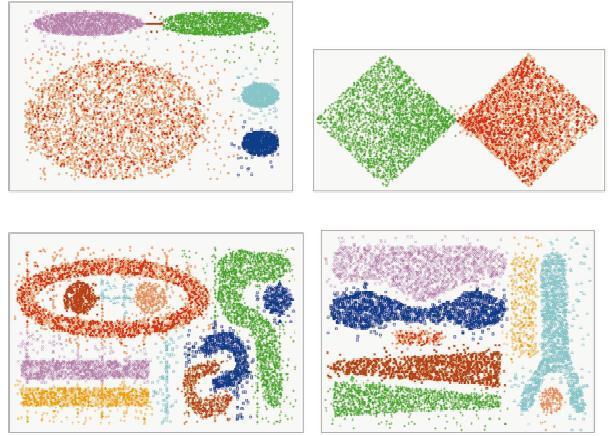
\includegraphics[width=0.55\textwidth]{img/cluster.jpeg}
\end{frame}

\begin{frame}{Probabilistic Hierarchical Clustering}
	\textbf{Algorithmic hierarchical clustering.}
	\begin{itemize}
		\item Nontrivial to choose a good distance measure.
		\item Hard to handle missing attribute values.
		\item Optimization goal not clear: heuristic, local search.
	\end{itemize}
	\textbf{Probabilistic hierarchical clustering.}
	\begin{itemize}
		\item Use probabilistic models to measure distances between
		      clusters.
		\item \textbf{\color{airforceblue}Generative model:}
		      \begin{itemize}
			      \item Regard the set of data objects to be clustered as a
			            sample of the underlying data-generation mechanism to be
			            analyzed.
		      \end{itemize}
		\item Easy to understand, same efficiency as algorithmic
		      agglomerative clustering method, can handle partially observed data.
		\item In practice, assume the generative models adopt
		      \textbf{\color{airforceblue}common distribution functions}, e.g.,
		      Gaussian distribution or Bernoulli distribution, governed by
		      parameters.
	\end{itemize}
\end{frame}

\begin{frame}{Generative Model (I)}
	\centering
	\begin{itemize}
		\item Given a set of $1$-D points $X = \{x_1, \ldots, x_n\}$ for
		      clustering analysis and assuming they are generated by a Gaussian
		      distribution:
		      \begin{align*}
			      N(\mu,\sigma) = \frac{1}{\sqrt{2 \pi \sigma^2}}
			      \exp\left({\frac{(\mathbf{x}-\mu)^2}{2\sigma^2}}\right).
		      \end{align*}
		\item The probability that a point $x_i \in X$ is generated by the
		      model:
		      \begin{align*}
			      P(x_i \vert \mu, \sigma) = \frac{1}{\sqrt{2\pi\sigma^2}} \exp\left(
			      \frac{(\mathbf{x_i}-\mu)^2}{2\sigma^2}\right).
		      \end{align*}
	\end{itemize}
\end{frame}

\begin{frame}{Generative Model (II)}
	\centering
	\begin{itemize}
		\item The likelihood that $X$ is generated by the model:
		      \begin{align*}
			      L(N(\mu,\sigma) \vert X) := P(X \vert \mu, \sigma) =
			      \prod_{i=1}^{n} \frac{1}{\sqrt{2\pi\sigma^2}} \exp\left(
			      \frac{(x_i-\mu)^2}{2\sigma^2}\right).
		      \end{align*}
		\item The task of learning the generative model: find the parameters
		      $\mu$ and $\sigma$, such that
		      \begin{align*}
			      N(\mu_0,\sigma_0) = \text{arg max}\left( L(N(\mu,\sigma)\vert X)
			      \right).
		      \end{align*}
	\end{itemize}
\end{frame}

\begin{frame}{A Probabilistic Hierarchical Clustering Algorithm (I)}
	\centering
	\begin{itemize}
		\item For a set of objects partitioned into $m$ clusters $C_1, \ldots,
			      C_m$,
		      the quality can be measured by:
		      \begin{align*}
			      Q(\{C_1, \ldots, C_m\}) = \prod_{i=1}^{m} P(C_i),
		      \end{align*}
		      where $P(C_i)$ is the maximum likelihood of $C_i$.
		\item Distance between clusters $C_i$ and $C_j$ can be computed as a
		      proximity measure:
		      \begin{align*}
			      d(C_i,C_j) = - \log \frac{P(C_i \cup C_j)}{P(C_i)P(C_j)}.
		      \end{align*}
	\end{itemize}
\end{frame}

\begin{frame}{A Probabilistic Hierarchical Clustering Algorithm (II)}
	\textbf{Algorithm: Progressively merge points and clusters}
	\begin{itemize}
		\item Input: $D = \{o_1, \ldots, o_n\}$: a dataset containing $n$
		      objects.
		\item Output: A hierarchy of clusters.
		\item Method:
		      \begin{itemize}
			      \item \texttt{Create cluster for each object $C_i = \{o_i\}$,
				            for $1 \leq i \leq n$}.
			      \item \textbf{For $i=1$ to $n$:}
			            \begin{itemize}
				            \item \texttt{Find a pair of clusters $C_i$ and $C_j$, such
					                  that}\\
				                  $C_i, C_j = \text{arg max}_{i \neq j} \left( \log\left(
						                  \frac{P(C_i \cup C_j)}{P(C_i)P(C_j)} \right) \right)$.
				            \item \textbf{If $\log\left( \frac{P(C_i \cup
							                  C_j)}{P(C_i)P(C_j)}\right) > 0$ then} \texttt{merge $C_i$
					                  and $C_j$},
				            \item \textbf{Else stop.}
			            \end{itemize}
		      \end{itemize}
	\end{itemize}
\end{frame}
